\documentclass[14pt,a4paper]{extarticle}
\usepackage[T1]{fontenc}
\usepackage[utf8]{inputenc}
\usepackage[scaled]{helvet}
\renewcommand{\familydefault}{\sfdefault}
\usepackage{amsmath}
\usepackage{sansmath}
\sansmath
\usepackage[a4paper,margin=2cm,top=1.6cm,bottom=1.4cm]{geometry}
\usepackage{tikz}
\usetikzlibrary{arrows.meta}
\pagestyle{empty}
% Zweite Seite: 5-mm-Kästchen, 1 cm Rand
\newcommand{\kaestchen}{\newpage\null
\begin{tikzpicture}[remember picture,overlay]
\begin{scope}[shift={(current page.south west)}]\draw[step=5mm, black!45, line width=0.3pt] (1cm,1cm) grid (20cm,28.5cm);\draw[black!45, line width=0.3pt] (1cm,1cm) rectangle (20cm,28.5cm);\end{scope}
\end{tikzpicture}}
\setlength{\parindent}{0pt}
\hyphenpenalty=10000

% Nur Schwarz und Grau, die Blätter werden schwarz-weiß kopiert.
% Merkblock: Begriff und Text links, Zeichnung rechts.
\newcommand{\bl}{0.5}
\newcommand{\block}[3]{%
\begin{minipage}[c]{\bl\textwidth}\raggedright{\Large\bfseries #1\par}\medskip #2\end{minipage}\hfill
\begin{minipage}[c]{\dimexpr0.97\textwidth-\bl\textwidth\relax}\centering #3\end{minipage}\par}

% Koordinatensystem: Kästchen 0,5 Einheiten wie im Buch. #1 bis #4 Fenster, #5 Zahlen auf der x-Achse, #6 auf der y-Achse.
\newcommand{\achsen}[6]{%
  \draw[black!22, line width=0.3pt, step=0.5] (#1,#3) grid (#2,#4);
  \draw[-{Stealth[length=2.2mm]}, line width=0.8pt] (#1,0) -- ({#2+0.45},0);
  \draw[-{Stealth[length=2.2mm]}, line width=0.8pt] (0,#3) -- (0,{#4+0.45});
  \node[below, font=\small] at ({#2+0.3},-0.05) {$x$};
  \node[left, font=\small] at (-0.05,{#4+0.3}) {$y$};
  \foreach \t in {#5} \draw[line width=0.6pt] (\t,0.1) -- (\t,-0.1) node[below=-1pt, font=\scriptsize] {$\t$};
  \foreach \t in {#6} \draw[line width=0.6pt] (0.1,\t) -- (-0.1,\t) node[left=-1pt, font=\scriptsize] {$\t$};
}
\tikzset{
  normal/.style={black!45, line width=1pt, dash pattern=on 4pt off 3pt},
  kurve/.style={black, line width=1.6pt},
  kurve2/.style={black!60, line width=1.6pt},
  pfeil/.style={-{Stealth[length=2.6mm,width=2.2mm]}, line width=1.4pt},
  lab/.style={fill=white, inner sep=1.2pt, font=\normalsize}
}

\renewcommand{\bl}{0.55}
\newcommand{\sk}{0.66cm}
\begin{document}

{\LARGE\bfseries Parabeln strecken, stauchen, verschieben\par}
\vspace{0.5cm}

\block{Strecken und Stauchen}{%
$f(x) = a\,x^2$\par\smallskip
$f(x) = 2x^2$: gestreckt\par
$g(x) = 0{,}5x^2$: gestaucht\par
$h(x) = -x^2$: nach unten offen\par\smallskip
$a$ positiv: nach oben offen\par
$a$ negativ: nach unten offen}{%
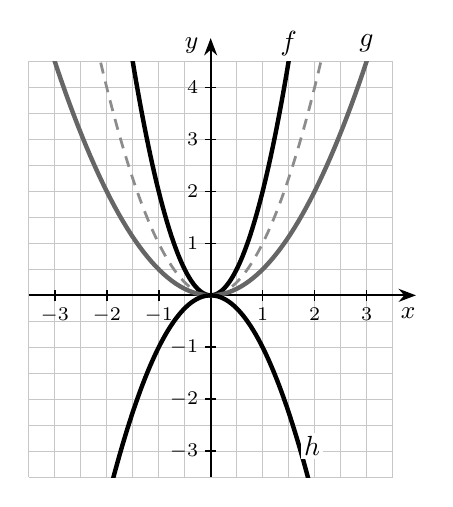
\begin{tikzpicture}[x=\sk,y=\sk]
  \achsen{-3.5}{3.5}{-3.5}{4.5}{-3,-2,-1,1,2,3}{-3,-2,-1,1,2,3,4}
  \begin{scope}\clip (-3.5,-3.5) rectangle (3.5,4.5);
    \draw[normal, domain=-2.2:2.2, samples=80] plot (\x, {\x*\x});
    \draw[kurve, domain=-1.55:1.55, samples=80] plot (\x, {2*\x*\x});
    \draw[kurve2, domain=-3.1:3.1, samples=80] plot (\x, {0.5*\x*\x});
    \draw[kurve, domain=-1.95:1.95, samples=80] plot (\x, {-\x*\x});
  \end{scope}
  \node[lab] at (1.5,4.85) {$f$};
  \node[lab] at (3.0,4.85) {$g$};
  \node[lab] at (1.95,-2.9) {$h$};
\end{tikzpicture}}

\vspace{0.35cm}

\block{Nach oben oder unten}{%
$f(x) = x^2 + e$\quad $S(0|e)$\par\smallskip
$f(x) = x^2 + 2$: 2 nach oben\par
$g(x) = x^2 - 3$: 3 nach unten}{%
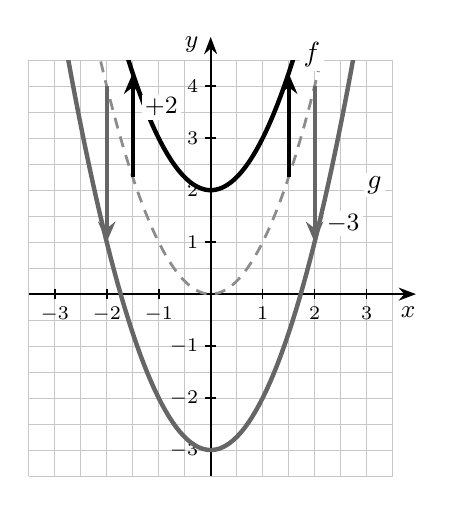
\begin{tikzpicture}[x=\sk,y=\sk]
  \achsen{-3.5}{3.5}{-3.5}{4.5}{-3,-2,-1,1,2,3}{-3,-2,-1,1,2,3,4}
  \begin{scope}\clip (-3.5,-3.5) rectangle (3.5,4.5);
    \draw[normal, domain=-2.2:2.2, samples=80] plot (\x, {\x*\x});
    \draw[kurve, domain=-1.6:1.6, samples=80] plot (\x, {\x*\x+2});
    \draw[kurve2, domain=-2.75:2.75, samples=80] plot (\x, {\x*\x-3});
  \end{scope}
  \draw[pfeil] (-1.5,2.25) -- (-1.5,4.25);
  \draw[pfeil] (1.5,2.25) -- (1.5,4.25);
  \draw[pfeil, black!60] (2,4) -- (2,1);
  \draw[pfeil, black!60] (-2,4) -- (-2,1);
  \node[lab, font=\small] at (2.55,1.35) {$-3$};
  \node[lab, font=\small] at (-0.95,3.6) {$+2$};
  \node[lab] at (1.95,4.6) {$f$};
  \node[lab] at (3.15,2.1) {$g$};
\end{tikzpicture}}

\vspace{0.35cm}

\block{Nach rechts oder links}{%
$f(x) = (x - d)^2$\quad $S(d|0)$\par\smallskip
$f(x) = (x - 2)^2$: 2 nach rechts\par
$g(x) = (x + 3)^2$: 3 nach links\par\smallskip
\textbf{Minus in der Klammer heißt nach rechts.}}{%
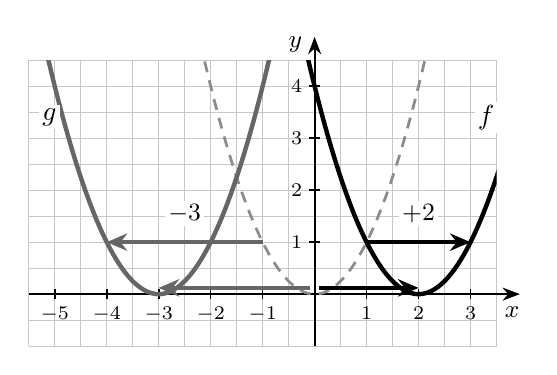
\begin{tikzpicture}[x=\sk,y=\sk]
  \achsen{-5.5}{3.5}{-1}{4.5}{-5,-4,-3,-2,-1,1,2,3}{1,2,3,4}
  \begin{scope}\clip (-5.5,-1) rectangle (3.5,4.5);
    \draw[normal, domain=-2.2:2.2, samples=80] plot (\x, {\x*\x});
    \draw[kurve, domain=-0.2:4.2, samples=80] plot (\x, {(\x-2)*(\x-2)});
    \draw[kurve2, domain=-5.2:-0.8, samples=80] plot (\x, {(\x+3)*(\x+3)});
  \end{scope}
  \draw[pfeil] (0.08,0.12) -- (2,0.12);
  \draw[pfeil, black!60] (-0.08,0.12) -- (-3,0.12);
  \draw[pfeil] (1,1) -- (3,1);
  \draw[pfeil, black!60] (-1,1) -- (-4,1);
  \node[lab, font=\small] at (2,1.55) {$+2$};
  \node[lab, font=\small] at (-2.5,1.55) {$-3$};
  \node[lab] at (3.3,3.4) {$f$};
  \node[lab] at (-5.1,3.4) {$g$};
\end{tikzpicture}}

\vspace{0.35cm}

\block{Scheitelpunktform}{%
$f(x) = a(x - d)^2 + e$\par
Scheitelpunkt $S(d|e)$\par\medskip
$f(x) = 2(x + 3)^2 + 2$\par\smallskip
$a = 2$: gestreckt, nach oben offen\par
$d = -3$: 3 nach links\par
$e = 2$: 2 nach oben, $S({-3}|2)$\par\smallskip
Von $S$ aus 1 nach rechts\par und $a$ nach oben.}{%
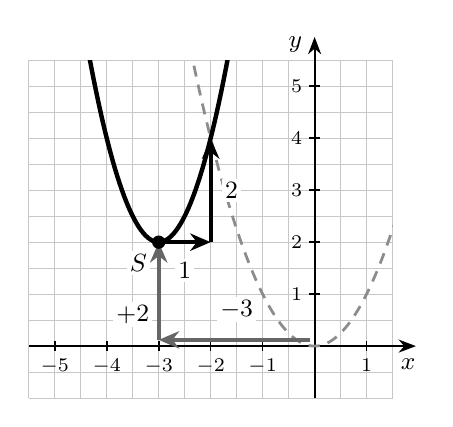
\begin{tikzpicture}[x=\sk,y=\sk]
  \achsen{-5.5}{1.5}{-1}{5.5}{-5,-4,-3,-2,-1,1}{1,2,3,4,5}
  \begin{scope}\clip (-5.5,-1) rectangle (1.5,5.5);
    \draw[normal, domain=-2.4:1.6, samples=80] plot (\x, {\x*\x});
    \draw[kurve, domain=-4.8:-1.2, samples=80] plot (\x, {2*(\x+3)*(\x+3)+2});
  \end{scope}
  \draw[pfeil, black!60] (-0.08,0.12) -- (-3,0.12);
  \draw[pfeil, black!60] (-3,0.12) -- (-3,2);
  \draw[pfeil] (-3,2) -- (-2,2);
  \draw[pfeil] (-2,2) -- (-2,4);
  \fill (-3,2) circle (2.4pt);
  \node[lab, font=\small] at (-1.5,0.7) {$-3$};
  \node[lab, font=\small] at (-3.5,0.6) {$+2$};
  \node[lab, font=\small] at (-2.5,1.45) {$1$};
  \node[lab, font=\small] at (-1.6,3.0) {$2$};
  \node[lab, font=\small, anchor=east] at (-3.15,1.6) {$S$};
\end{tikzpicture}}

\vfill

{\Large\bfseries Aufgaben im Heft\par}
\medskip
Buch S.\,\rule{1.5cm}{0.4pt} Nr.\,\rule{5cm}{0.4pt}

\kaestchen
\end{document}
